\section{Consultar Datos Personales}

Un usuario necesita saber su información personal y los roles a los que pertenece, de esta manera él tendrá un conocimiento de todos los datos que tiene asociados a su cuenta.

\subsubsection{Procedimiento}
\begin{enumerate}
	
	\item Da clic en el icono \textbf{Datos Personales} de la pantalla \textbf{Menú Principal del Doctor}.

		\begin{figure}[!htbp]			\hypertarget{fig:mpDoctorCD}{\hspace{1pt}}
		\begin{center}
			\includegraphics[height=0.4\textheight]{images/Iconos/Advertencia}
			\caption{Menú Principal del Doctor}
			\label{fig:mpDoctorCD}
		\end{center}
	\end{figure}

	\item Se mostrará la pantalla \textbf{Datos Personales}. 
	\newpage
	\begin{figure}[!htbp]			
		\hypertarget{fig:DatosPersonales}{\hspace{1pt}}
		\begin{center}
			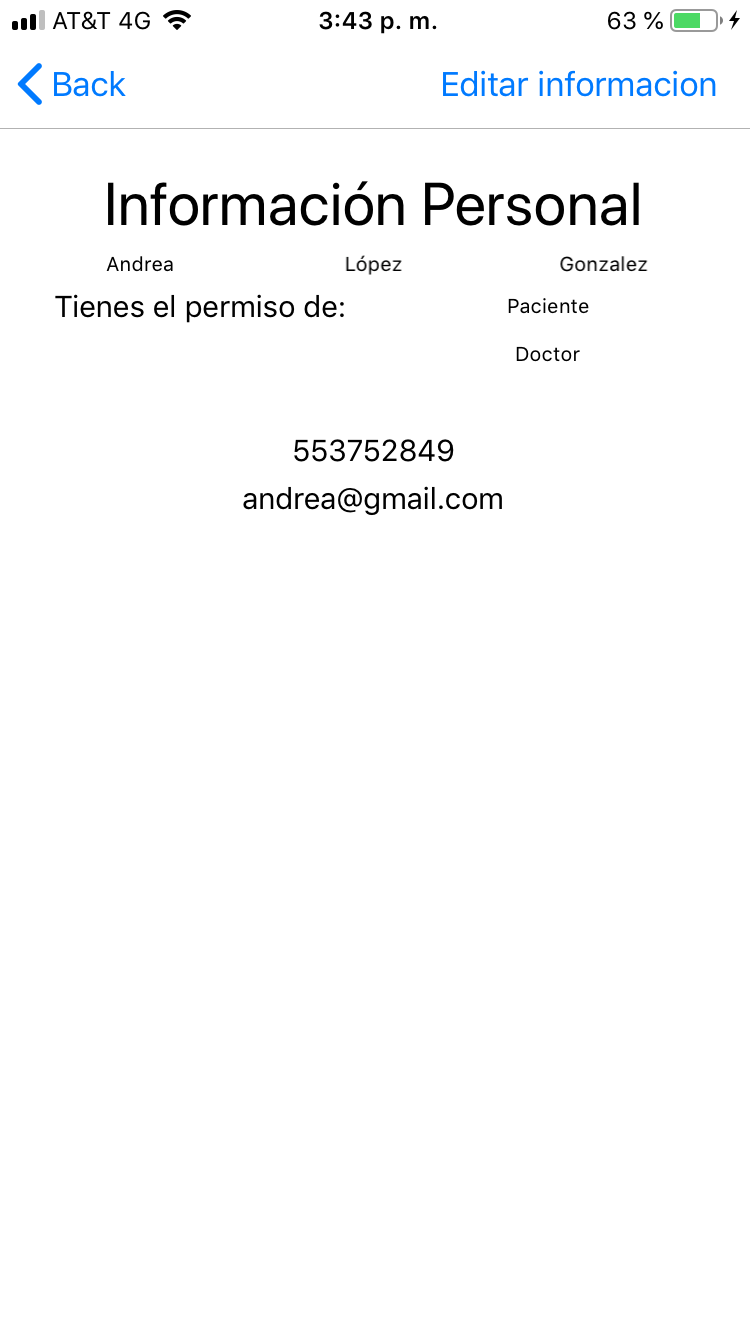
\includegraphics[height=0.4\textheight]{Doctor/ConsultarDP/images/DatosPersonales}
			\caption{Datos Personales}
			\label{fig:DatosPersonales}
		\end{center}
	\end{figure}

	\item Consulta los datos personales y luego da clic en el botón \textbf{Back} para regresar a la pantalla \ref{fig:mpDoctorCD} \textbf{Menú Principal del Doctor}.


\end{enumerate}

